\documentclass[11pt]{article}

% Preamble: Core Packages
\usepackage[utf8]{inputenc}
\usepackage[T1]{fontenc}
\usepackage{amsmath}
\usepackage{amssymb}
\usepackage{array}    % For p{}, m{}, b{} column types if needed
\usepackage{graphicx}
\usepackage{bookmark}
\usepackage{comment}
\usepackage{booktabs} % For professional tables
\usepackage[margin=1in]{geometry} % Sensible margins
\usepackage[labelfont=bf]{caption} % For caption styling
\usepackage{tabularx}    % For tables with adjustable width columns
\usepackage{array}       % For more advanced column formatting (like m{} or p{})
\newcolumntype{L}{>{\raggedright\arraybackslash}X} % Defines a new 'L' column type
\usepackage{makecell}    % For line breaks in table cells/headers (\thead)
\usepackage{siunitx}     % For SI units (optional, but good practice for numbers with units)
\usepackage{caption}     % For better control over captions
\usepackage[numbers, sort&compress]{natbib}
\usepackage{hyperref}
% Hyperref setup
\hypersetup{
    colorlinks=true,
    linkcolor=blue,
    filecolor=magenta,
    urlcolor=cyan,
    pdftitle={A Biomimetic Model for Schlieren Vision}, % Add PDF metadata
    pdfauthor={Daniel Sandner}
}

% Title and Author
\title{A Biomimetic Model for Schlieren Vision:\\Hypothetical Anatomy and Functional Morphology}
\author{{Daniel Sandner}\thanks{Corresponding author: Daniel Sandner, Independent Researcher, 100 Scientific Visions Initiative, \href{news@sandner.art}{news@sandner.art}}} % Add author information here if available

\date{\today} % Or \date{} for no date

\begin{document}

\maketitle

\bigskip\noindent\rule{\linewidth}{0.4pt}\bigskip

\begin{abstract}
This paper explores the theoretical possibility of biomimetic Schlieren vision – a sensory modality that would enable organisms to perceive subtle density variations in transparent media, such as air and water. While no known organism possesses a dedicated Schlieren visual system, we demonstrate that such a capability is biophysically plausible, predictable, and could evolve through natural selection under appropriate environmental pressures. Our primary contribution is the development of hypothetical anatomical and functional morphological models, inspired by diverse animal groups (insects, amphibians, and birds), which detail how biological structures could amplify and detect the minute optical effects of density variations. We first establish the fundamental principles of Schlieren optics and the core requirements for any biological system capable of detecting density gradients: a mechanism for amplifying the tiny refractive index variations, a means of detecting the amplified signal (likely through mechanoreceptors), and a mechanism for spatial resolution. We then present a general mathematical framework that captures these principles. Building upon this foundation, we propose three distinct, speculative anatomical adaptations inspired by diverse animal groups: a modified insect compound eye with layered chitin in elongated ommatidia, a specialized amphibian nictitating membrane with a pressure-sensitive fluid chamber, and a novel adaptation of the avian pecten oculi incorporating a network of fluid-filled channels. Each model represents a different strategy for achieving amplification and detection, highlighting the potential for convergent evolution. We discuss the evolutionary advantages of Schlieren vision in various contexts, including movement through fluids, predator-prey interactions, and navigation. We also propose experimental designs to test these hypothetical mechanisms and to investigate potential precursors of Schlieren sensing in existing organisms. Finally, we discuss the broad implications of this research for biomimetic sensor technology, highlighting potential applications in underwater exploration, atmospheric monitoring, medical diagnostics, and other fields. This work provides a theoretical outline for understanding the potential for density-gradient-based vision and inspires the development of novel sensing technologies.
\end{abstract}

\noindent\textbf{Keywords:} Biomimetics, Theoretical Biology, Comparative Morphology, Schlieren Vision, Density Gradient Sensing, Sensory Evolution, Mechanoreception, Optical Physics, Evolutionary Biology, Hypothetical Sensory Models.


\newpage

\section{Introduction}

The ability to perceive the subtle density fluctuations that permeate our world, invisible to the human eye, would open up a new dimension of sensory experience. While we readily perceive the world through variations in light intensity and wavelength (color), a hidden landscape of density variations remains largely inaccessible to our senses. This paper explores the tantalizing possibility of a visual system based on density gradients – a form of "density vision" – and the biophysical principles that could make it a reality. From navigating murky waters to detecting camouflaged objects, the capacity to visualize density gradients would revolutionize sensing technologies across diverse fields, including robotics, medicine, and environmental monitoring. The question, then, is not simply \textit{whether} such a sensory modality is possible, but rather \textit{how} biological systems might evolve to achieve it. Specifically, what are the fundamental biophysical constraints and design principles that govern the possibility of biological systems capable of detecting and interpreting subtle variations in refractive index, and how might these principles be realized through diverse anatomical adaptations?

\begin{figure}[htbp]
    \centering
    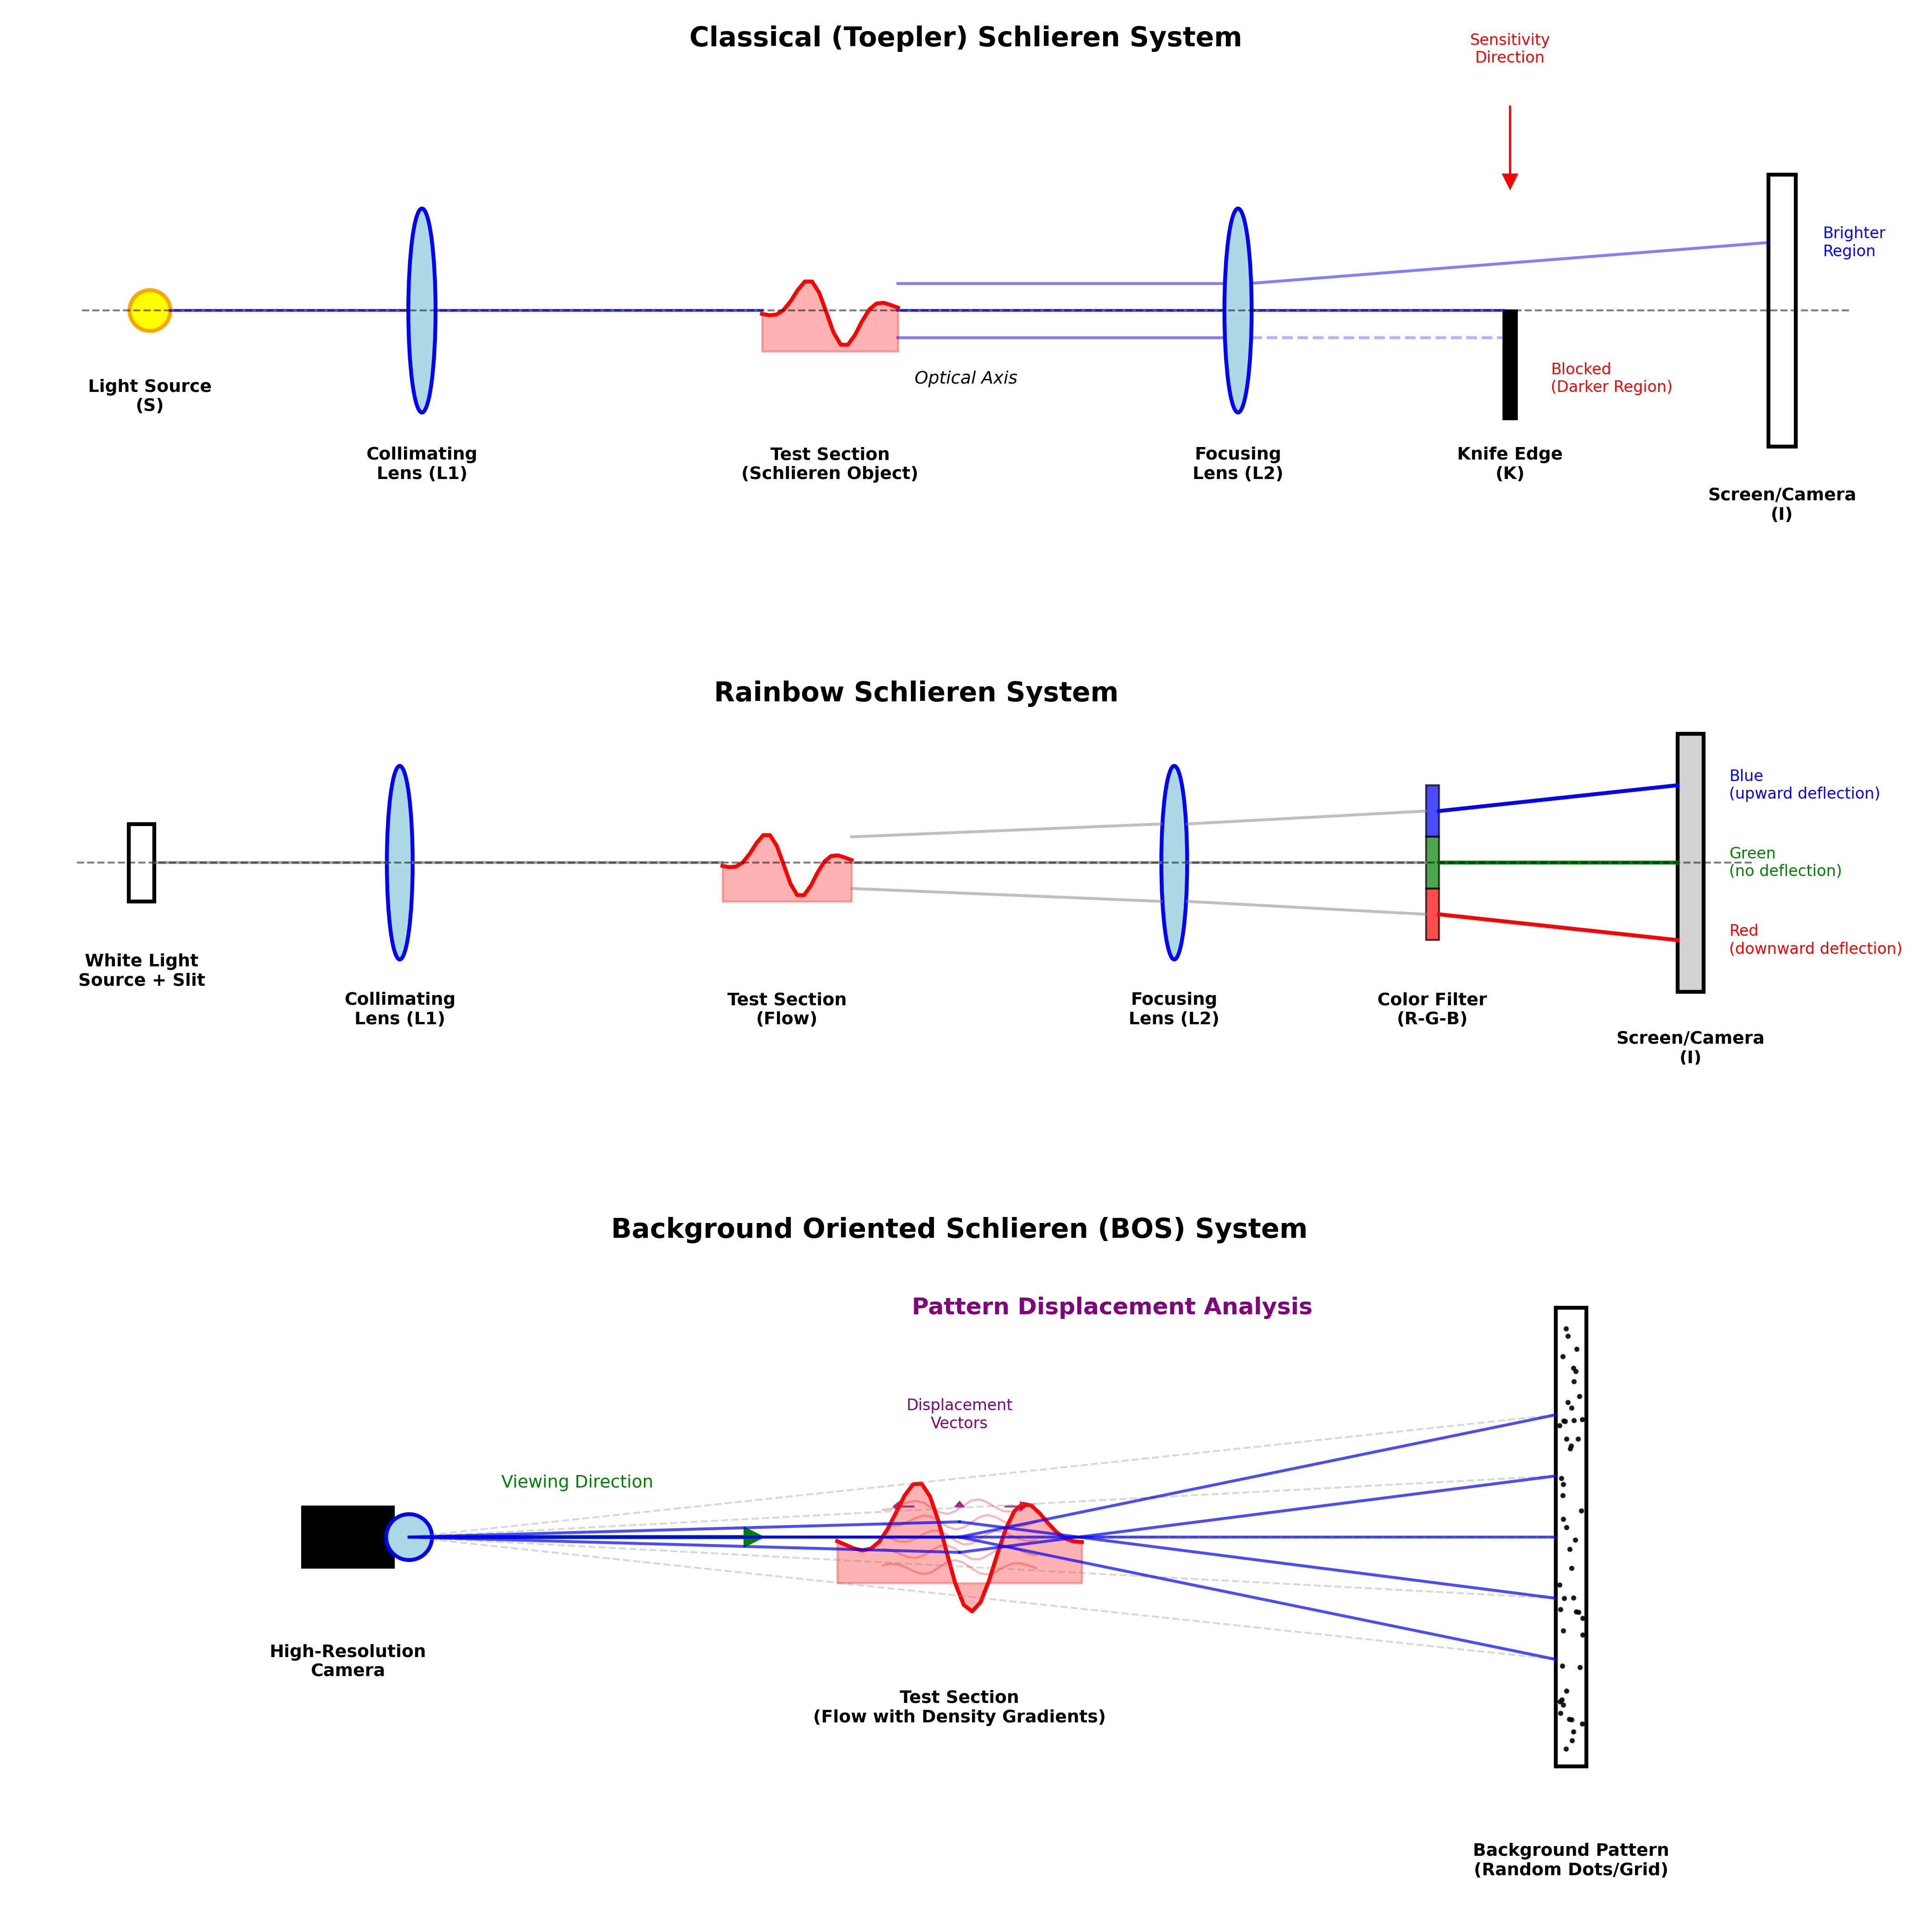
\includegraphics[width=0.99\textwidth]{figures/classical_schlieren_system.png} % Replace with your actual filename
    \caption{Schematic overview of common optical Schlieren imaging techniques.
    \textbf{(Top)} Classical (Toepler) Schlieren system, utilizing a knife-edge to visualize density gradients as brightness variations.
    \textbf{(Middle)} Rainbow Schlieren system, employing a color filter to produce a color-coded map of density gradients.
    \textbf{(Bottom)} Background Oriented Schlieren (BOS) system, which analyzes the apparent distortion of a background pattern to quantify density fields.
    Further details and biomimetic considerations for these techniques are discussed in Section~\ref{sec:schlieren_principles_biomimetic}.} % Assumes the new subsection has this label
    \label{fig:schlieren_systems_overview}
\end{figure}

To answer this question, we must first understand the underlying physics. Schlieren optics, a set of techniques used to visualize density variations in transparent media \cite{Settles2001Schlieren}, relies on a fundamental principle: light bends when it encounters a change in refractive index \cite{Hecht2017Optics}. The refractive index of a material is, in turn, directly related to its density \cite{Gladstone1863Refraction, Hecht2017Optics}; denser materials generally have higher refractive indices. Therefore, when light passes through a region with a density gradient (a gradual change in density), it is deflected from its original path. The magnitude of this deflection is proportional to the \textit{change} in refractive index, and thus to the density gradient. However, the challenge lies in the fact that \textit{subtle} density variations, such as those caused by temperature differences in air or salinity gradients in water, produce \textit{extremely small} changes in refractive index, and consequently, very small light deflections. Traditional Schlieren imaging techniques, such as the Z-type configuration or single-mirror setups \cite{Settles2001Schlieren}, overcome this challenge using precise optical arrangements and sensitive detectors. These methods serve as a technological proof-of-concept, demonstrating that density variations \textit{can} be visualized.

The biological world, however, often finds ingenious solutions to seemingly insurmountable challenges. The diversity of sensory modalities across the animal kingdom is a testament to the power of natural selection to shape sensory systems finely tuned to their environment. From the echolocation of bats and dolphins \cite{Au1993DolphinSonar}, which use sound waves to "see" in the dark, to the electroreception of sharks and rays \cite{Bullock2005Electroreception}, which detect the weak electrical fields produced by other organisms, nature abounds with examples of sensory systems that detect subtle environmental cues imperceptible to humans. Even within the realm of vision, we find remarkable adaptations, such as the infrared vision of snakes, which allows them to "see" the heat emitted by their prey, or the polarization vision of some insects, which enables them to navigate using the polarization patterns of skylight. Might there also be, or have been, organisms capable of sensing subtle differences of density in their surrounding? The lateral line system of fish \cite{Dijkgraaf1963LateralLine}, which detects pressure waves and water movements using mechanoreceptors, and the statocysts of cnidarians \cite{Budelmann1992InvertebrateHearing}, which sense gravity, hint at the possibility of rudimentary density sensing. Although these systems are not specifically designed for Schlieren vision, they demonstrate that biological systems \textit{can} evolve to detect subtle mechanical cues related to density variations.

This paper explores the fundamental principles of biomimetic Schlieren vision, proposing a general mechanics for how biological systems could detect and interpret density gradients. We first outline the core requirements for any such system, including mechanisms for amplification, detection, and spatial resolution. We then present a general mathematical model that captures the essential physics. Finally, we will explore how these principles might be realized through diverse anatomical adaptations in three hypothetical animal models: a modified insect compound eye, a specialized amphibian nictitating membrane, and a novel adaptation of the avian pecten oculi. This comparative approach highlights the versatility of the underlying principles and suggests potential avenues for the development of bio-inspired sensing technologies.

% Add this label to the subsection for referencing from the figure caption
\subsection{Schlieren Imaging Principles and Biomimetic Considerations}
\label{sec:schlieren_principles_biomimetic}

The visualization of otherwise invisible density gradients in transparent media is achieved through various optical techniques collectively known as Schlieren imaging. These methods exploit the fundamental principle that light rays bend (refract) when passing through regions of varying refractive index, which are directly correlated with density changes. Understanding these established techniques provides a foundation for conceptualizing how biological systems might evolve analogous sensory capabilities. Figure~\ref{fig:schlieren_systems_overview} illustrates three common Schlieren modalities.


The \textbf{Classical (Toepler) Schlieren system} (Figure~\ref{fig:schlieren_systems_overview}, Top) \cite{Settles2001Schlieren} typically employs a point or slit light source, collimating optics, a test section where the density gradient (Schlieren object) resides, focusing optics, and a sharp cutoff device (like a knife-edge) positioned at the focal plane of the focusing optics. Light rays deflected by density gradients are differentially blocked or passed by the knife-edge, resulting in an image where these gradients appear as variations in brightness or shadow. The sensitivity is directional, typically perpendicular to the knife-edge.

     \textbf{\textit{Biomimetic Note:}}\textit{ While a direct biological analog with discrete external optical components is not likely, the core principle of amplifying angular deflections and using a differential cutoff could be realized within integrated biological structures. For instance, modified photoreceptive elements or internal anatomical features within an elongated sensory unit could act as distributed knife-edges or phase filters. Some laboratory Schlieren systems utilize a single focusing mirror with the test object placed in front of it (e.g., single-mirror or Z-fold systems with the object in a folded path), effectively creating a long interaction length. A biological counterpart might involve internal reflective layers (akin to a tapetum lucidum) within a compact organ to fold the optical path, allowing light to interact with the surrounding medium over an extended effective distance before encountering a detection/cutoff mechanism.}

The \textbf{Rainbow Schlieren system} (Figure~\ref{fig:schlieren_systems_overview}, Middle) \cite{Howes1984Rainbow, Settles2001Schlieren} is a variation that often uses a white light source and replaces the knife-edge with a multi-segment color filter (e.g., red-green-blue) at the focal plane. The degree and direction of light deflection determine which color segment the light passes through, rendering the density gradients as a color-coded map.

     \textbf{\textit{Biomimetic Note:}}\textit{ While complex, the principle of spectral filtering based on deflection angle is conceivable. Some organisms possess wavelength-specific photoreceptors or filtering pigments. A biological rainbow Schlieren might involve an array of mechanoreceptors or photoreceptors tuned to respond differently based on the angle (and thus effective wavelength or intensity after passing through a biological "filter") of light that has been spectrally dispersed by a prism-like biological structure or by diffraction from fine gratings after interacting with density gradients.}

The \textbf{Background Oriented Schlieren (BOS) system} (Figure~\ref{fig:schlieren_systems_overview}, Bottom) \cite{Raffel2018PIV} offers a computationally intensive but optically simpler approach. It involves imaging a known, often structured or random, background pattern through the transparent medium containing density gradients. Refraction caused by these gradients leads to apparent distortions or displacements of the background pattern. These displacements are quantified using image correlation techniques (such as those adapted from Particle Image Velocimetry) \cite{Raffel2018PIV}, allowing for the reconstruction of the density field.

     \textbf{\textit{Biomimetic Note:}}\textit{ BOS is perhaps the most directly analogous to a potential evolutionary pathway for a rudimentary form of density gradient perception. An organism with high-resolution vision could evolve neural mechanisms to detect subtle, correlated distortions or "shimmering" of a familiar background pattern when viewed through a transparent medium with density fluctuations. This requires sophisticated image processing but leverages existing visual acuity. It doesn't require specialized internal Schlieren optics like a knife-edge, but rather the interpretation of how external density fields distort the image of the environment formed by a conventional eye. The "object in focus in front of an inverted mirror" principle doesn't directly map here, as BOS relies on viewing a background *through* the density field \cite{Settles2017Review}.}

Beyond these common methods, other Schlieren-related techniques exist, such as phase-contrast imaging, interferometry (e.g., Mach-Zehnder), and shadowgraphy \cite{Settles2001Schlieren}. Shadowgraphy, the simplest, visualizes second spatial derivatives of the refractive index and relies on light redistribution without a knife-edge; it is sensitive to sharp gradients. While these more specialized techniques also offer insights into visualizing phase objects, the core principles of light deflection, optical path manipulation, and differential detection remain central to understanding the potential biophysical basis for any form of evolved Schlieren vision. Our exploration focuses on biomimetic adaptations drawing inspiration primarily from the fundamental mechanisms demonstrated by the classical, rainbow, and BOS approaches.

\section{Biomimetic Principles of Schlieren Vision}

Before delving into specific anatomical examples, we will establish the theoretical requirements that \textit{any} biological system must satisfy to achieve Schlieren vision. These requirements stem from the inherent challenges of detecting the subtle refractive index variations associated with small density gradients.

\begin{table}[htbp]
\centering
\caption{Common Environmental Density Gradient Sources and Estimated Detection Thresholds. Example data sources for profile concepts: oceanic data \cite{Talley2011Oceanography}, atmospheric conditions \cite{ISO1975StandardAtmosphere, Stull1988BoundaryLayer}.}
\label{tab:gradient_sources}
\scriptsize % This table has more content, might need smaller font
\begin{tabularx}{\textwidth}{@{}l L c c L L@{}}
\toprule
\thead{Environment} & \thead{Gradient Source} & \thead{Typical $\Delta\rho$} & \thead{Corresponding $\Delta n$} & \thead{Detection\\Advantage} & \thead{Biological\\Relevance} \\
\midrule
\textbf{Aquatic} & Temperature gradients & $10^{-3} - 10^{-1}$ kg/m$^3$ & $10^{-6} - 10^{-4}$ & Thermocline navigation & Fish migration, feeding \\
\addlinespace

& Salinity gradients & $10^{-2} - 10^{0}$ kg/m$^3$ & $10^{-5} - 10^{-3}$ & Halocline detection & Estuarine adaptation \\
\addlinespace

& Turbulence mixing & $10^{-4} - 10^{-2}$ kg/m$^3$ & $10^{-7} - 10^{-5}$ & Current detection & Energy-efficient swimming \\
& Biogenic mixing & $10^{-5} - 10^{-3}$ kg/m$^3$ & $10^{-8} - 10^{-6}$ & Prey/predator detection & Foraging, predator avoidance \\
\addlinespace
\textbf{Aerial} & Thermal columns & $10^{-3} - 10^{-1}$ kg/m$^3$ & $10^{-6} - 10^{-4}$ & Soaring efficiency & Energy conservation \\
& Humidity gradients & $10^{-4} - 10^{-2}$ kg/m$^3$ & $10^{-7} - 10^{-5}$ & Weather prediction & Migration timing \\
\addlinespace
& Wind shear & $10^{-4} - 10^{-2}$ kg/m$^3$ & $10^{-7} - 10^{-5}$ & Turbulence avoidance & Flight stability \\
& Boundary layers & $10^{-5} - 10^{-3}$ kg/m$^3$ & $10^{-8} - 10^{-6}$ & Obstacle detection & Navigation \\
\bottomrule
\end{tabularx}
\end{table}

\subsection{Core Requirements}

\subsubsection{Amplification}
The refractive index changes caused by subtle density variations in air or water are exceedingly small. Consequently, the deflection of light rays passing through these gradients is also minuscule, far below the detection threshold of typical biological photoreceptors. Therefore, the first and most critical requirement for a biological Schlieren system is a mechanism to \textit{amplify} these tiny refractive index variations into a detectable signal. This amplification must significantly increase the angular deviation of light rays before they reach the sensory cells.

\subsubsection{Detection}
Once the refractive index variations have been amplified, the system requires a mechanism to \textit{detect} the resulting changes in light direction or intensity. Given the mechanical nature of density gradients (pressure differences), the most plausible candidates for this role are \textit{mechanoreceptors}. These specialized sensory cells are exquisitely sensitive to mechanical deformation, converting tiny forces or displacements into electrical signals that can be processed by the nervous system.

\subsubsection{Spatial Resolution}
To be truly useful, a Schlieren vision system must not only detect density gradients but also determine their \textit{location} in space. This requires a mechanism for \textit{spatial resolution}, allowing the organism to distinguish between density variations in different parts of its visual field. This could be achieved through an array of individual sensing units (like the ommatidia in a compound eye) or through a scanning mechanism that samples different regions of the environment sequentially.

\subsection{General Mathematical Framework}

The fundamental physics underlying Schlieren vision is governed by Snell's Law \cite{Hecht2017Optics}, which describes the refraction (bending) of light at the interface between two media with different refractive indices:
\[n_1\sin(\theta_1) = n_2\sin(\theta_2)\]
where $n_1$ and $n_2$ are the refractive indices of the two media, and $\theta_1$ and $\theta_2$ are the angles of incidence and refraction, respectively (measured relative to the normal to the interface).

The refractive index ($n$) of a material is, in turn, related to its density ($\rho$). For gases, the relationship is approximately linear:
\[n \approx 1 + K\rho\]
where $K$ is the Gladstone-Dale constant \cite{Gladstone1863Refraction}, which depends on the specific gas and the wavelength of light. For liquids, the relationship can be more complex, but a similar principle applies: changes in density generally lead to changes in refractive index.

For the small angles of deflection typically involved in Schlieren vision, we can use the small angle approximation: $\sin(\theta) \approx \theta$ (in radians). Applying this approximation to Snell's Law, we get:
\[n_1\theta_1 \approx n_2\theta_2\]

Now, consider a light ray passing through a region with a gradual change in refractive index (and thus density). The ray will be continuously deflected as it traverses this gradient. The \textit{total} angular deflection ($\Delta\theta$) will depend on the \textit{magnitude} of the refractive index change ($\Delta n$) and the \textit{path length} ($L$) over which the change occurs.

To capture the combined effect of all the anatomical features that contribute to amplifying the signal, we introduce a \textit{general amplification factor} ($A$). This factor represents the ratio of the final angular deflection of the light ray (after passing through the specialized sensory structure) to the initial angular deflection that would occur in the absence of any amplification mechanism. The specific form of $A$ will depend on the particular biological implementation (e.g., the length and refractive index profile of an insect ommatidium, the geometry and fluid properties of an amphibian nictitating membrane).

The minimum detectable density change ($\Delta\rho_{\text{min}}$) can then be expressed in terms of $A$ and the minimum detectable angular deflection of the sensory cells ($\Delta\theta_{\text{min}}$):
\[\Delta\rho_{\text{min}} \approx \frac{\Delta\theta_{\text{min}}}{K \cdot A \cdot L}\]
Here, $\Delta\theta_{\text{min}}$ is determined by the sensitivity of the mechanoreceptors. This equation highlights the key factors influencing the sensitivity of a biological Schlieren system:
\begin{itemize}
    \item \textbf{Amplification Factor ($A$):} A larger amplification factor allows for the detection of smaller density changes.
    \item \textbf{Sensor Sensitivity ($\Delta\theta_{\text{min}}$):} More sensitive mechanoreceptors (smaller $\Delta\theta_{\text{min}}$) improve sensitivity.
    \item \textbf{Path Length ($L$):} Longer path amplifies changes.
    \item \textbf{Gladstone-Dale Constant ($K$):} Properties of the material.
\end{itemize}
In the following sections, we will explore how these general principles are manifested in three distinct hypothetical biological models, each employing a different anatomical strategy to achieve Schlieren vision.

\bigskip\noindent\rule{\linewidth}{0.4pt}\bigskip

\section{Anatomical Adaptations and Hypothetical Features}

Having established the core requirements and general mathematical framework for biomimetic Schlieren vision, we now explore how these principles might be realized through diverse anatomical adaptations in three hypothetical animal models: a modified insect compound eye, a specialized amphibian nictitating membrane, and a novel adaptation of the avian pecten oculi. Each model represents a distinct strategy for amplifying and detecting subtle refractive index variations, showcasing the versatility of natural selection in achieving similar functional outcomes through different structural means.

\subsection{Insect Model (Modified Compound Eye)}

Insects, with their remarkable diversity of visual adaptations, offer a compelling starting point for exploring biomimetic Schlieren vision. We propose a modification of the compound eye \cite{Land2012AnimalEyes}, a structure already known for its high spatial resolution and wide field of view. The key adaptation lies in specialized ommatidia, the individual units that make up the compound eye.

\subsubsection{Key Anatomical Features:}
Instead of the typical conical shape, these "Schlieren ommatidia" would be extremely elongated and narrow, resembling thin, slightly curved tubes. This increased length is important for amplifying the refractive effect. The outer cornea would focus light into the ommatidium, but immediately beneath it would lie a series of \textit{very} thin layers of chitin (refractive index $n \approx 1.52-1.58$ \cite{Tsai2008ChitinOptical}), each with a \textit{slightly different refractive index}. This layered structure forms a miniature, biological "Schlieren apparatus" within each ommatidium. The rhabdom \cite{Land2012AnimalEyes}, the light-sensitive part of the ommatidium, would be clear and contain specialized \textit{mechanoreceptors} instead of traditional photoreceptor pigments. These mechanoreceptors would be arranged in a grid-like pattern along the rhabdom, sensitive to tiny deformations caused by the bending of light.

\subsubsection{Functional Mechanism:}
As light passes through the layered chitin, the small differences in refractive index between adjacent layers cause a cumulative bending effect. This is analogous to the way a stack of lenses with slightly different focal lengths can focus light. The longer the ommatidium and the greater the number of layers, the greater the amplification (higher $A$ in our general model). The bending light exerts a tiny pressure on the rhabdom walls, deforming the mechanoreceptors. The pattern of mechanoreceptor activation encodes the direction and magnitude of the light deflection, providing information about the density gradient.

\subsubsection{Potential Advantages and Disadvantages:}
This design offers potentially high spatial resolution, due to the large number of individual ommatidia. However, the sensitivity might be limited by the small diameter of each ommatidium and the challenges of fabricating such a precisely layered structure biologically. The energy cost of building and maintaining such elongated ommatidia could also be significant. However, especially in the case of insects, it would provide big advantage (coincidentally, Schlieren imaging was in fact already used to study vortex structures around hawkmoths \cite{Liu2018SchlierenHawkmoth}).

\begin{figure}[htbp]
    \centering
    % Ensure this filename matches the image that includes panels A, B, C, D, and E
    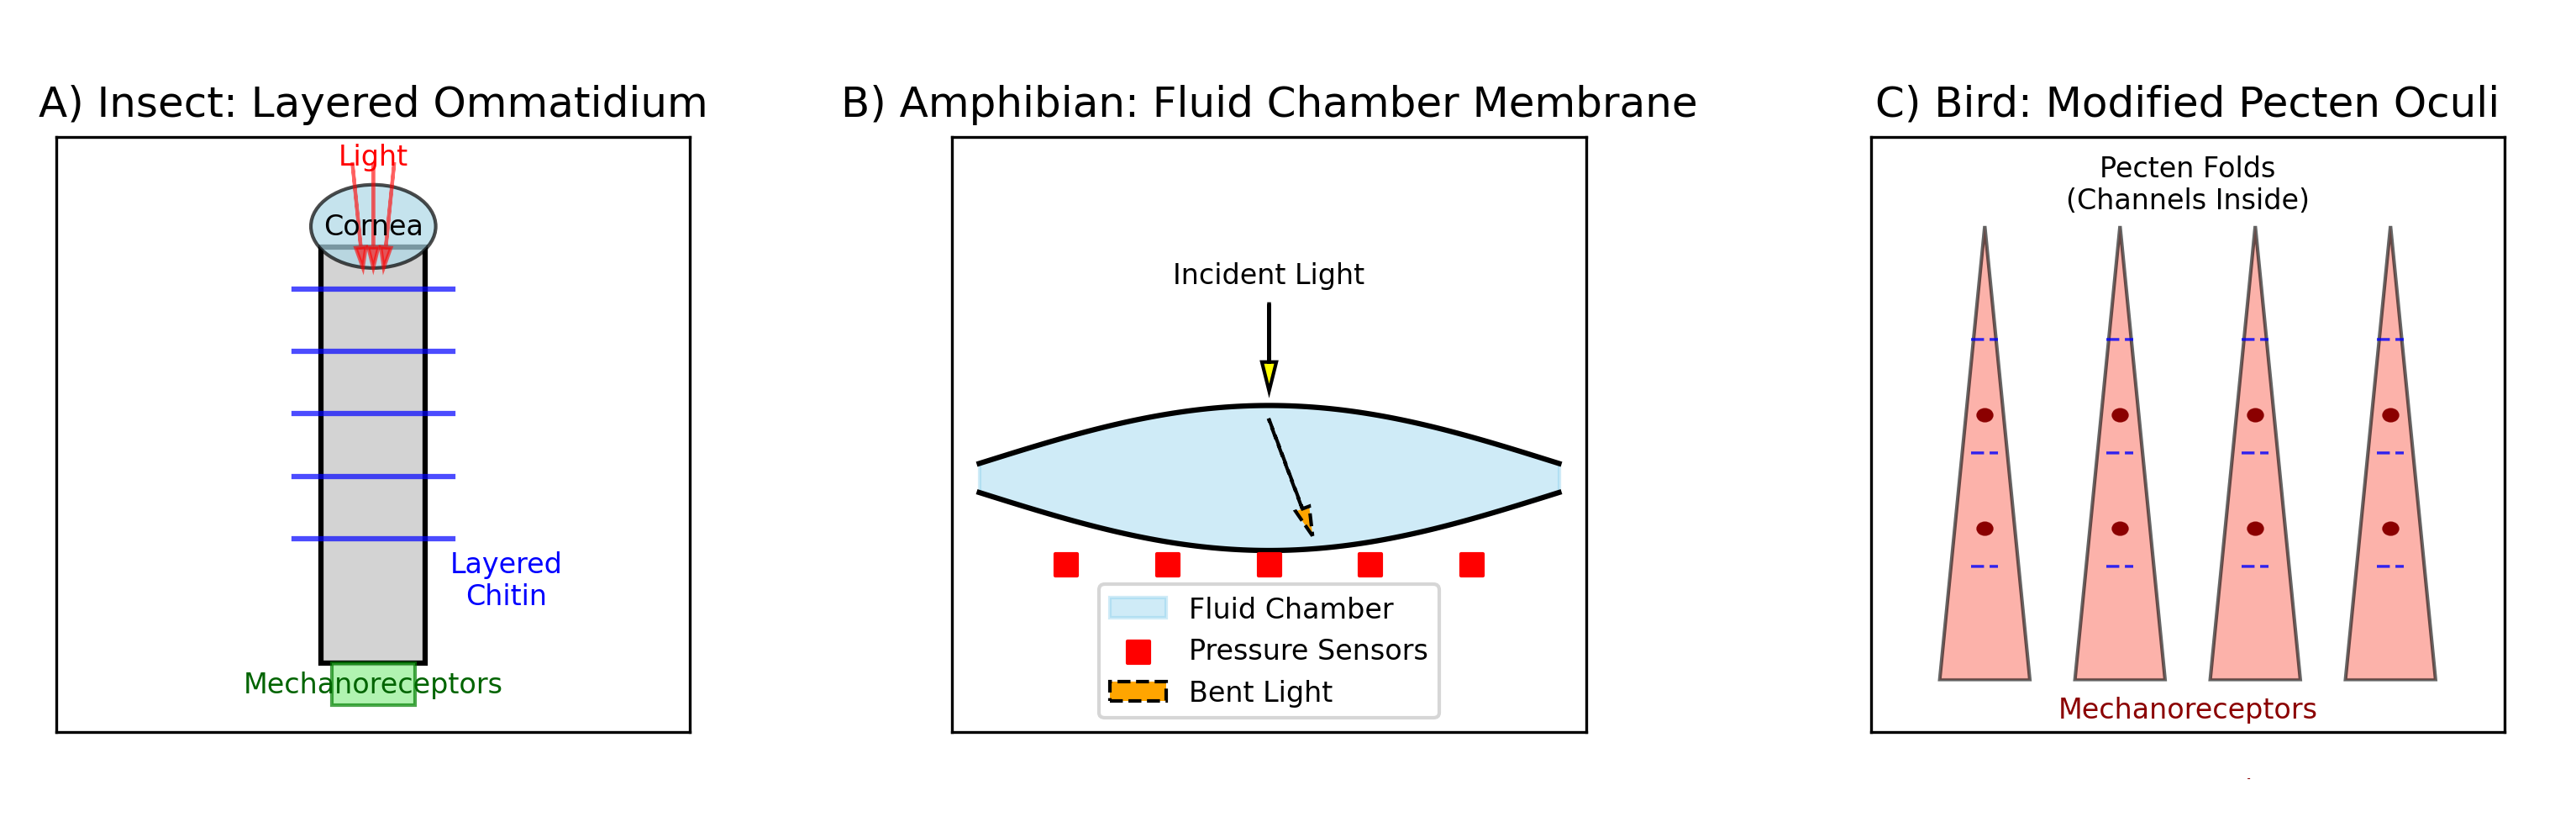
\includegraphics[width=\textwidth]{figures/figure5_biomimetic_schlieren_corrected.png}
    \caption{\textbf{Biomimetic implementation strategies and evolution:} Conceptual models of hypothetical biomimetic Schlieren vision systems and their evolutionary context. Panels A-C illustrate distinct anatomical strategies for amplifying subtle light deflections caused by refractive index gradients and detecting these changes via mechanoreception.
    \textbf{(A)} Insect Model: A specialized, elongated ommatidium from a compound eye. Incident light passes through the cornea and a series of thin, layered chitin structures with minutely differing refractive indices, causing cumulative light bending (amplification). Mechanoreceptors at the rhabdom's base detect the resulting pressure or displacement.
    \textbf{(B)} Amphibian Model: A modified nictitating membrane incorporating a biconvex, fluid-filled chamber. External density variations alter the refractive index of the contained fluid, which in turn modifies the path of transmitted light. This change in light path creates differential pressure on an underlying array of mechanosensitive cells (pressure sensors).
    \textbf{(C)} Avian Model: An adaptation of the avian pecten oculi. This model proposes a network of microfluidic channels within the pecten's vascularized folds, filled with a refractive-index-sensitive fluid. Light deflections within these channels due to external aerial density gradients would be detected by integrated mechanoreceptors.
    All anatomical schematics are conceptual and not to scale.}
    \label{fig:biomimetic_strategies_evolution} % Keep a consistent label
\end{figure}


\subsection{Amphibian Model (Modified Nictitating Membrane)}

Amphibians, with their aquatic and terrestrial lifestyles, often possess a nictitating membrane \cite{Walls1942VertebrateEye} – a transparent or translucent third eyelid that protects the eye and keeps it moist. We propose a modification of this membrane to achieve Schlieren vision.

\subsubsection{Key Anatomical Features:}
The core of this modified nictitating membrane would be a sealed chamber filled with a specialized fluid. This fluid would have a high refractive index sensitivity to density changes – meaning that even small changes in the surrounding water's density would significantly alter the fluid's refractive index. Beneath the fluid chamber, a thin layer of \textit{pressure-sensitive cells} (mechanoreceptors) would be embedded in the membrane. Tiny muscles could control the membrane's position and potentially adjust the pressure within the fluid chamber, "tuning" its sensitivity.

\subsubsection{Functional Mechanism:}
As the amphibian moves through water with varying density (e.g., due to temperature or salinity differences), the refractive index of the surrounding water changes. This, in turn, alters the refractive index of the fluid within the chamber. The resulting change in the light path through the chamber creates a pressure difference on the underlying mechanoreceptors. The pattern of mechanoreceptor activation provides a map of the density gradients.

\subsubsection{Potential Advantages and Disadvantages:}
This design could offer high sensitivity, due to the highly responsive fluid and the direct coupling between pressure changes and mechanoreceptor activation. However, the spatial resolution might be lower than the insect model, as it depends on the density of mechanoreceptors within the membrane, rather than on individual, tightly packed ommatidia. Maintaining the precise composition and pressure of the fluid could also be a challenge.

\subsection{Bird/Flying Animal Model (Modified Pecten Oculi)}

Birds, renowned for their exceptional visual acuity, possess a unique structure within their eye called the pecten oculi \cite{Meyer1977AvianEye}. Its exact function remains debated, but it's thought to be involved in nourishing the retina. We propose a novel adaptation of the pecten to achieve Schlieren vision, particularly suited for detecting density gradients in air.

\subsubsection{Key Anatomical Features:}
We hypothesize that the pecten, in this modified form, would contain a network of tiny, interconnected channels filled with a fluid or gel that is highly sensitive to refractive index changes. This network would be richly supplied with mechanoreceptors, sensitive to subtle changes in pressure or flow within the channels. The pecten's position within the eye, near the optic nerve, would place it in the path of light entering the eye.

\subsubsection{Functional Mechanism:}
As the bird flies through air with varying density (e.g., due to thermals or turbulence), the refractive index of the surrounding air changes. This, in turn, alters the refractive index of the fluid or gel within the pecten's channels. The resulting changes in light refraction within the channels create tiny pressure or flow variations, which are detected by the mechanoreceptors. The complex, folded structure of the pecten could amplify these subtle changes.

\subsubsection{Potential Advantages and Disadvantages:}
This design could potentially be integrated with the existing visual system, providing a dual-purpose sensory structure. However, the mechanism is the most speculative of the three, and the developmental challenges of creating such a finely tuned structure within the pecten would be significant. The spatial resolution would likely depend on the complexity of the channel network and the density of mechanoreceptors.

\subsection{Comparative Analysis}

These three models represent distinct, yet fundamentally similar, approaches to biomimetic Schlieren vision. All three rely on the core principles of amplification and mechanoreceptor detection, but they employ different anatomical strategies to achieve these goals.

\begin{table}[htbp]
\centering
\caption{Enhanced Comparative Analysis of Proposed Biomimetic Schlieren Models. (Refractive index of chitin $n=1.52-1.58$ \cite{Tsai2008ChitinOptical})}
\label{tab:enhanced_comparative}
\scriptsize
\begin{tabularx}{\textwidth}{@{}L L L L L@{}}
\toprule
\thead{Feature} & \thead{Insect Model} & \thead{Amphibian Model} & \thead{Bird Model} & \thead{Performance Metrics} \\
\midrule
\textbf{Amplification Mechanism} & Layered chitin ($n=1.52-1.58$) & Fluid chamber ($n=1.33-1.45$) & Channel network ($n=1.35-1.42$) & Amplification factor: $10^2-10^4$ \\
\addlinespace % Adds space here
\textbf{Detection Method} & Mechanoreceptors in rhabdom & Pressure-sensitive cells & Mechanoreceptors in pecten & Sensitivity: $10^{-6}$ to $10^{-4} \Delta n$ \\
\addlinespace % Adds space here

\textbf{Spatial Resolution} & High (\num{1000}--\num{10000} ommatidia) & Moderate (\num{100}--\num{1000} cells) & Variable (depends on pecten) & Angular resolution: $0.1-10^\circ$ \\
\addlinespace % Adds space here

\textbf{Temporal Resolution} & Fast ($1-10$ ms) & Moderate ($10-100$ ms) & Moderate ($5-50$ ms) & Response time range \\
\addlinespace % Adds space here

\textbf{Sensitivity} & Moderate ($10^{-5} \Delta n$) & High ($10^{-6} \Delta n$) & Moderate ($10^{-5} \Delta n$) & Minimum detectable change \\
\addlinespace % Adds space here

\textbf{Energy Requirements} & Moderate (structural maintenance) & Low (passive system) & High (active circulation) & Relative metabolic cost \\
\addlinespace % Adds space here

\textbf{Environmental Tolerance} & High (robust exoskeleton) & Moderate (aquatic limitation) & High (aerial adaptation) & Operating range \\
\addlinespace % Adds space here

\textbf{Developmental Feasibility} & Moderate (chitin layering) & High (membrane modification) & Low (complex integration) & Evolutionary likelihood \\
\addlinespace % Adds space here

\textbf{Biomimetic Potential} & High (microfabrication) & Very High (microfluidics) & Moderate (complex geometry) & Engineering implementability \\
\bottomrule
\end{tabularx}
\end{table}

The insect model, with its highly ordered array of ommatidia, offers the potential for high spatial resolution, allowing for detailed mapping of density gradients. The amphibian model, with its fluid-filled chamber, prioritizes sensitivity, making it well-suited for detecting subtle density changes in aquatic environments. The bird model, while the most speculative, suggests a way to integrate Schlieren vision with an existing, highly developed visual system. These trade-offs highlight the diverse ways in which natural selection could shape the evolution of Schlieren vision, depending on the specific ecological niche and sensory demands of the organism. The optimal design would likely depend on the specific environment and the organism's behavioral needs.

\bigskip\noindent\rule{\linewidth}{0.4pt}\bigskip

\section{Evolutionary Considerations}

The emergence of Schlieren vision in any organism would be driven by natural selection, favoring individuals with an enhanced ability to detect and interpret density gradients in their environment. The specific evolutionary pathways and selective pressures would likely vary depending on the organism's lifestyle and ecological niche.

\subsection{Evolutionary Pathways}

It is unlikely that a fully formed Schlieren sensory system would arise \textit{de novo}. Instead, it would likely evolve through a series of incremental steps, each providing a small but significant advantage. Potential starting points, as mentioned earlier, could include:
\begin{itemize}
    \item \textbf{Mechanoreceptor Sensitivity:} Existing mechanoreceptors, sensitive to touch, pressure, or vibration \cite{Keil1997InsectMechanoreceptors, Hudspeth1989EarWorks}, could become more refined and specialized for detecting subtle pressure differences associated with density gradients.
    \item \textbf{Fluid-Filled Structures:} Structures already containing fluids (e.g., statocysts \cite{Budelmann1992InvertebrateHearing}, the eye itself \cite{Walls1942VertebrateEye}) could evolve fluids with greater refractive index sensitivity to density changes.
    \item \textbf{Optical Modifications:} Existing optical structures (e.g., lenses \cite{Hecht2017Optics}, corneas) could be modified to enhance the bending of light in response to refractive index variations.
\end{itemize}
In the case of the insect model, the evolution of elongated ommatidia with layered chitin could be driven by a gradual increase in ommatidial length and the refinement of chitin deposition processes, leading to a more pronounced amplification of refractive index changes. For the amphibian model, the nictitating membrane, already providing protection and lubrication, could evolve a more specialized fluid and a denser array of pressure-sensitive cells. In the bird model, the pecten oculi, with its existing vascular supply and proximity to the retina, could gradually develop a network of fluid-filled channels and associated mechanoreceptors.

\subsection{Advantages and Trade-offs}

\begin{figure}[htbp]
    \centering
    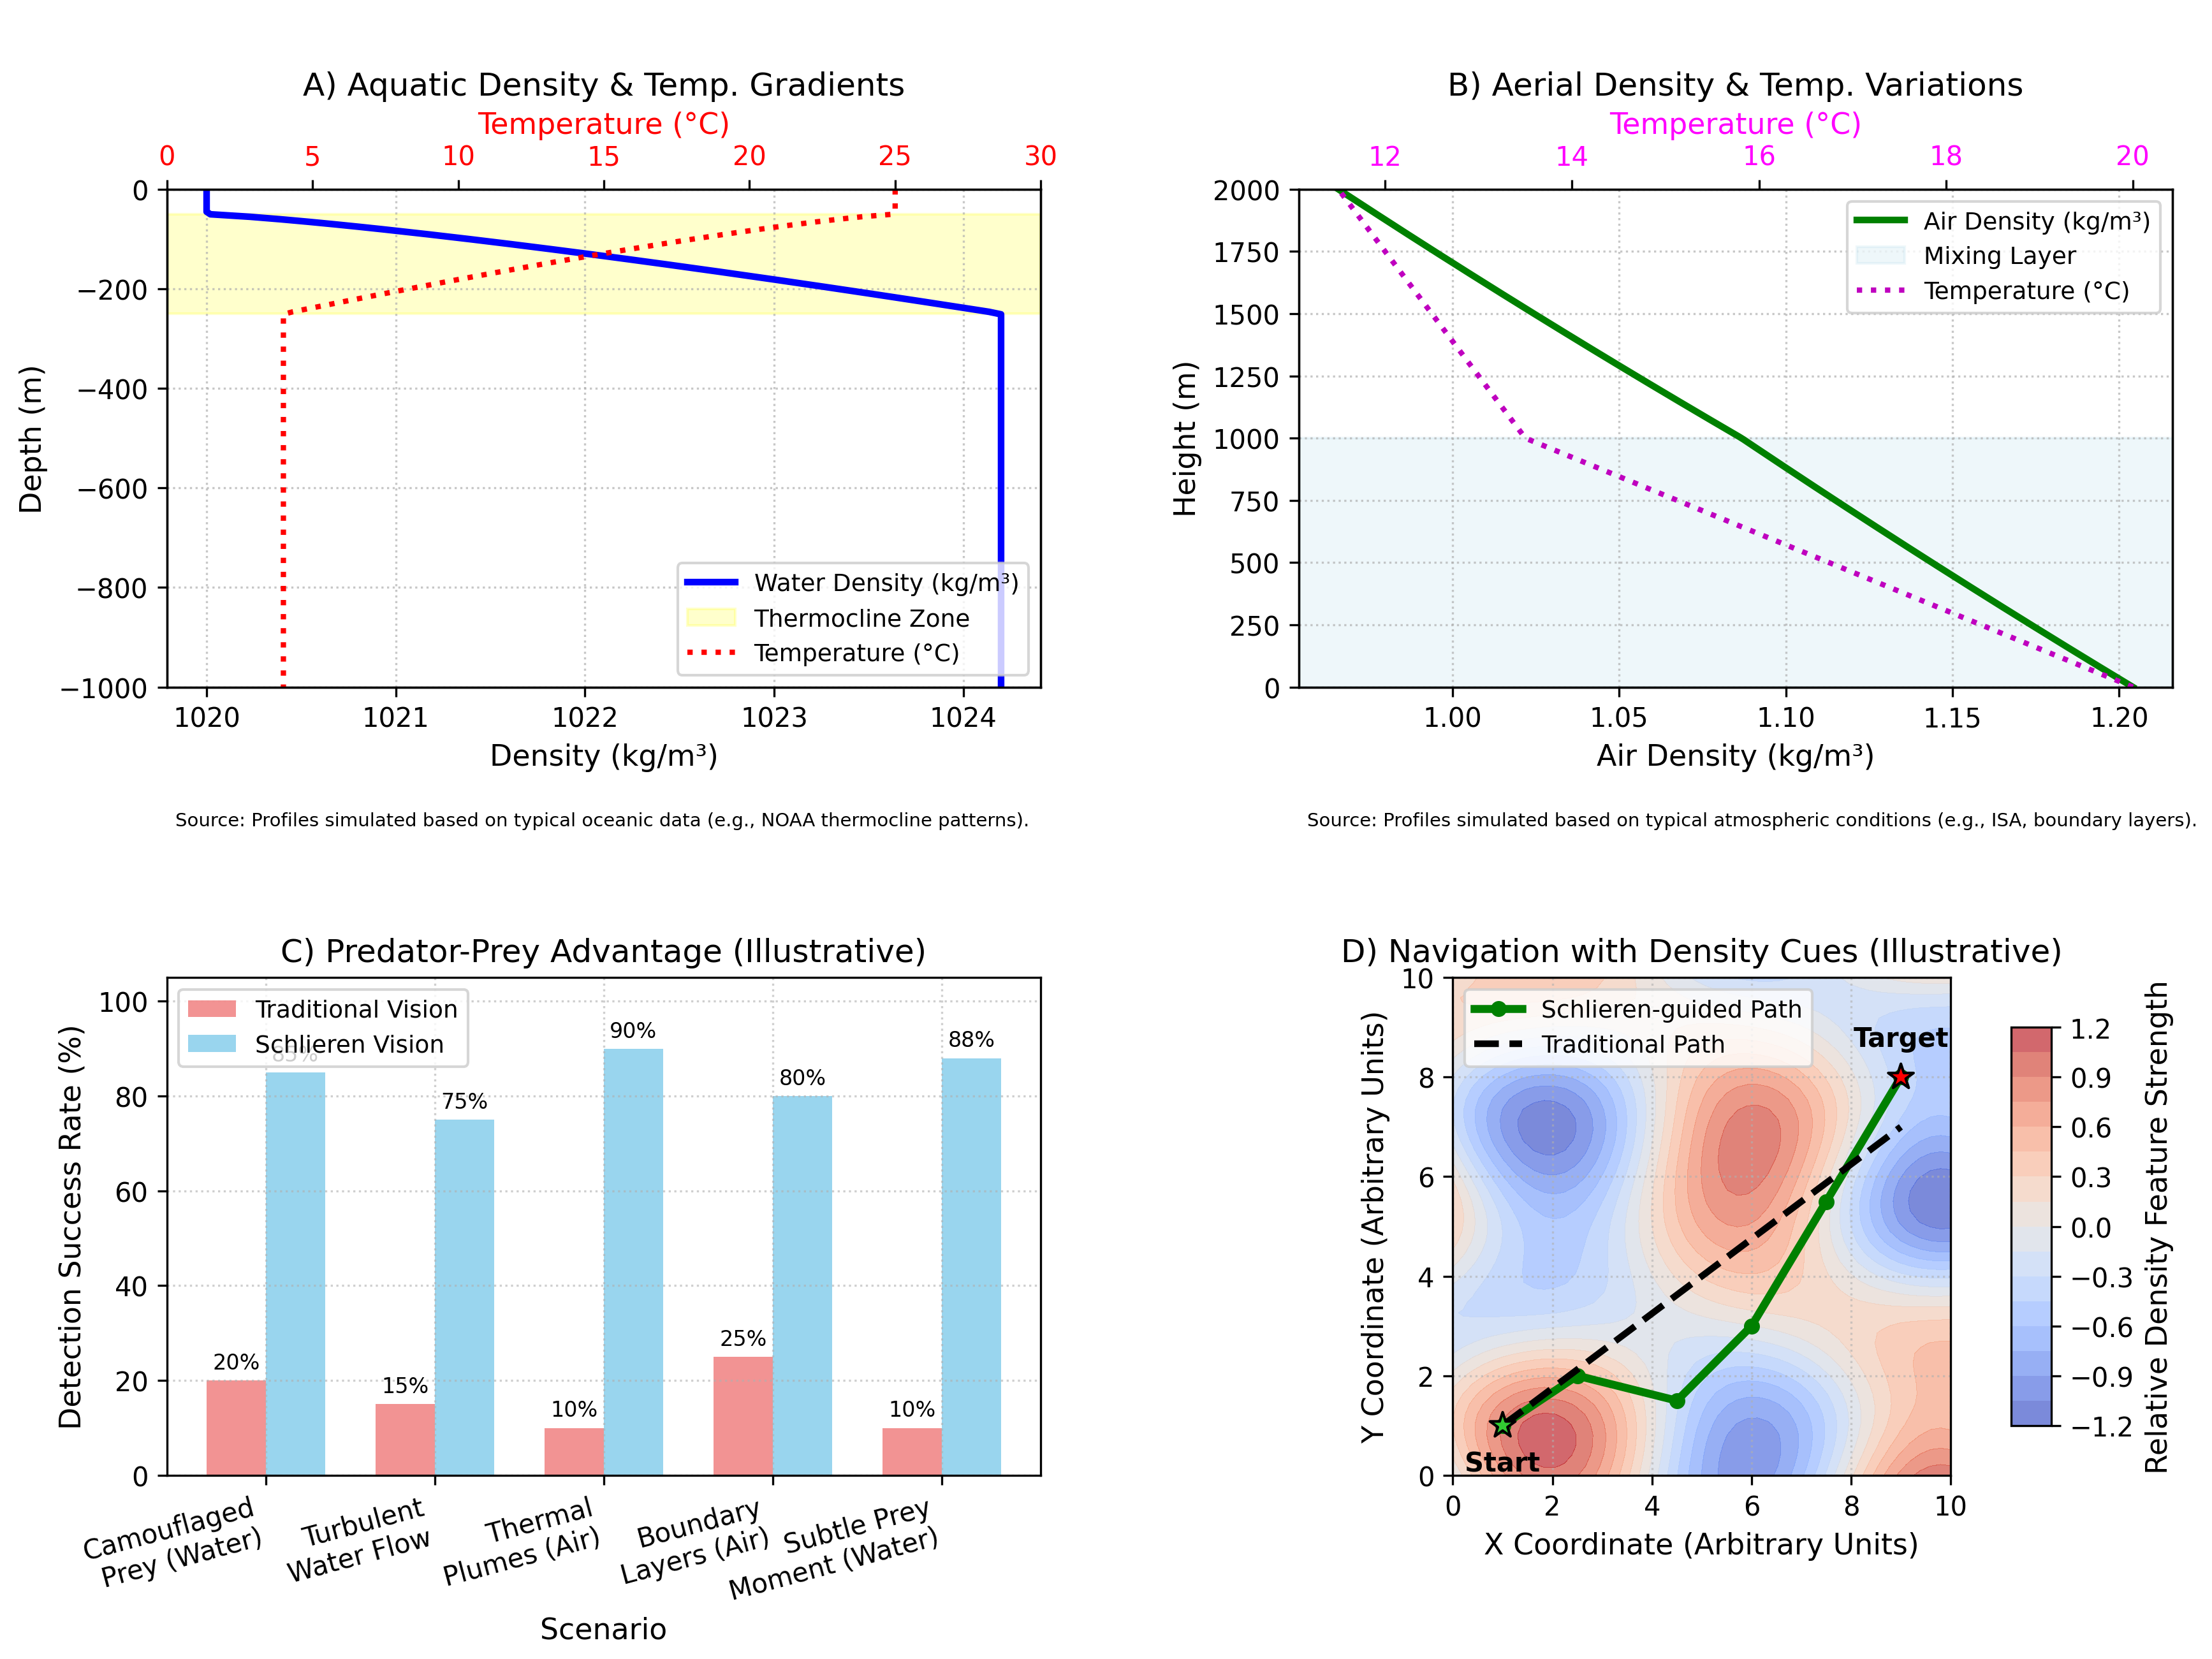
\includegraphics[width=0.95\textwidth]{figures/figure4_environmental_applications.png} % Assumes this is the image for Fig 4 from draft
    \caption{Potential environmental applications and selective advantages of biomimetic Schlieren vision.
    \textbf{(A)} Simulated aquatic density and temperature profiles, highlighting a thermocline zone where significant density gradients occur. Such features are common in oceans and lakes and influence organismal distribution and behavior. Source: Profiles simulated based on typical oceanic data patterns (e.g., NOAA thermocline patterns \cite{Talley2011Oceanography}, with gradients sharpened for illustration).
    \textbf{(B)} Simulated aerial density and temperature variations with height, showing an atmospheric mixing layer. Density gradients in air, such as thermals or boundary layers, are critical for avian flight and insect dispersal. Source: Profiles simulated based on typical atmospheric conditions (e.g., International Standard Atmosphere \cite{ISO1975StandardAtmosphere}, boundary layer concepts \cite{Stull1988BoundaryLayer}).
    \textbf{(C)} Illustrative comparison of detection success rates for traditional vision versus hypothetical Schlieren vision in various predator-prey scenarios, suggesting a significant advantage for Schlieren sensing in detecting camouflaged or subtly moving targets.
    \textbf{(D)} Conceptual depiction of navigation using density cues. A Schlieren-guided path (green) exploits perceived density features (color contour) for not the shortest but potentially more efficient or secure travel compared to a traditional path (black dashed), relevant for migration or foraging.}
    \label{fig:environmental_applications}
\end{figure}

The evolutionary advantages of Schlieren vision are numerous and diverse, as discussed previously. These include:
\begin{itemize}
    \item \textbf{Enhanced Movement:} Efficient navigation through fluids, exploiting currents and thermals, and improved maneuverability.
    \item \textbf{Predation:} Penetrating camouflage, detecting subtle movements of prey, and predicting prey trajectories.
    \item \textbf{Defense:} Detecting approaching predators, even if camouflaged, and executing effective evasion maneuvers.
    \item \textbf{Navigation:} Creating "density maps" of the environment, aiding in orientation and finding resources.
    \item \textbf{Potential Communication:} (More speculative) Using subtle density signals for mating displays, territorial marking, or warning signals.
\end{itemize}
However, the evolution of Schlieren vision would also involve trade-offs:
\begin{itemize}
    \item \textbf{Energy Cost:} Building and maintaining specialized sensory structures, and processing the resulting information, would require energy. This cost must be outweighed by the benefits.
    \item \textbf{Reduced Acuity in Other Modalities:} An eye optimized for Schlieren vision might be less sensitive to light intensity or color, potentially compromising other visual functions.
    \item \textbf{Vulnerability:} The specialized sensory structures (e.g., elongated ommatidia, fluid-filled chambers) might be more vulnerable to damage.
\end{itemize}
The specific balance of these advantages and trade-offs would determine whether Schlieren vision evolves in a particular lineage and the specific form it takes.

\bigskip\noindent\rule{\linewidth}{0.4pt}\bigskip

\section{Experiment Design}

While we cannot directly experiment on hypothetical organisms, we can propose experimental designs that \textit{could} be used to test the proposed mechanisms, \textit{if} such organisms existed. We can also propose experiments to investigate potential precursors of Schlieren sensing in \textit{existing} organisms.

\subsection{Experiments on Hypothetical Schlieren Systems}

For each of the three models (insect, amphibian, bird), we could propose experiments involving:
\begin{itemize}
    \item \textbf{Controlled Density Gradients:} Creating precisely controlled density gradients in the organism's environment (air or water). This could be achieved using:
    \begin{itemize}
        \item \textbf{Layered Fluids:} Creating layers of fluids with slightly different salinities or temperatures.
        \item \textbf{Heated Elements:} Creating localized temperature gradients in air or water.
        \item \textbf{Microfluidic Devices:} Using microfluidic channels to generate precisely controlled gradients.
    \end{itemize}
    \item \textbf{Physiological Recordings:} Measuring the response of the sensory structures to these gradients. This could involve:
    \begin{itemize}
        \item \textbf{Microelectrodes:} Inserting tiny electrodes into the ommatidia (insect), nictitating membrane (amphibian), or pecten (bird) to record the activity of mechanoreceptors.
        \item \textbf{High-Speed Video Microscopy:} Observing the movement of the ommatidia, nictitating membrane, or pecten in response to density changes.
        \item \textbf{Optical Coherence Tomography (OCT) \cite{Huang1991OCT}:} A non-invasive imaging technique that could potentially be used to visualize the internal structure of the sensory organs and detect any changes in response to density gradients.
    \end{itemize}
    \item \textbf{Behavioral Assays:} Observing the organism's behavior in response to density gradients. This could involve:
    \begin{itemize}
        \item \textbf{Tracking Movement:} Analyzing the organism's movement patterns in the presence of different gradients.
        \item \textbf{Choice Tests:} Giving the organism a choice between environments with different density gradients.
        \item \textbf{Predator-Prey Interactions:} Observing how the presence of density gradients affects hunting or evasion behavior.
    \end{itemize}
    \item \textbf{Controls:} All experiments would require appropriate controls to rule out other factors that might influence the results (e.g., visual cues, temperature changes unrelated to density gradients).
\end{itemize}

\subsection{Experiments on Potential Precursors}

We can also propose experiments to investigate potential precursors of Schlieren sensing in \textit{existing} organisms:
\begin{itemize}
    \item \textbf{Lateral Line System (Fish, Amphibian Larvae) \cite{Dijkgraaf1963LateralLine}:}
    \begin{itemize}
        \item Expose fish or amphibian larvae to carefully controlled density gradients (e.g., using layers of water with slightly different salinities).
        \item Use high-speed video microscopy to observe the movement of the neuromasts (hair cells).
        \item Use microelectrodes to record the activity of the neuromasts.
    \end{itemize}
    \item \textbf{Cnidarian Statocysts \cite{Budelmann1992InvertebrateHearing}:}
    \begin{itemize}
        \item Examine statocysts under a microscope while manipulating the density of the surrounding fluid.
        \item Potentially use micro-Schlieren techniques to visualize any light bending within the statocyst.
    \end{itemize}
    \item \textbf{Insect Mechanoreceptors \cite{Keil1997InsectMechanoreceptors}:}
    \begin{itemize}
        \item Expose insects to carefully controlled air density gradients (e.g., using heated air).
        \item Observe their behavior.
        \item Use electrophysiological recordings to measure the activity of campaniform sensilla or hair-plate sensilla.
    \end{itemize}
    \item \textbf{Bird Pecten Oculi \cite{Meyer1977AvianEye}:}
    \begin{itemize}
        \item Perform detailed anatomical studies of the pecten using micro-CT scanning and other imaging techniques.
        \item Potentially use micro-Schlieren techniques to visualize any fluid flow or light bending within the pecten.
        \item Examine the response to different density gradients.
    \end{itemize}
\end{itemize}
These experiments, while challenging, would provide valuable insights into the potential for density gradient detection in existing biological systems \cite{Merzkirch1987FlowVisualization} and could shed light on the evolutionary pathways that might lead to Schlieren vision.

\bigskip\noindent\rule{\linewidth}{0.4pt}\bigskip


\section{Discussion}

This paper has presented a theoretical framework for biomimetic Schlieren vision, exploring the fundamental biophysical principles and proposing three distinct anatomical adaptations that could enable organisms to detect and interpret density gradients. While these models are speculative, they are grounded in established scientific principles and draw inspiration from the remarkable diversity of sensory systems found in nature.

\begin{table}[htbp]
\centering
\caption{Biophysical Requirements and Biological Precedents for Density Gradient Sensing. Sensitivity ranges are indicative \cite{Hudspeth1989EarWorks, Keil1997InsectMechanoreceptors, Budelmann1992InvertebrateHearing}. Refractive indices from \cite{Hecht2017Optics, Walls1942VertebrateEye, Land2012AnimalEyes, Stavenga2003CompoundEyeOptics}.}
\label{tab:bio_requirements}
\footnotesize % Adjust font size for the table if needed (e.g., \footnotesize, \small, \normalsize)
\begin{tabularx}{\textwidth}{@{}L L L c L@{}} % Use tabularx for width control
\toprule
\thead{Requirement} & \thead{Biological\\Precedent} & \thead{Organism\\Examples} & \thead{Sensitivity Range} & \thead{Potential\\for Schlieren\\Adaptation} \\
\midrule
\textbf{Mechano-receptor Sensitivity} & Hair cells (lateral line) \cite{Dijkgraaf1963LateralLine} & Fish, amphibian larvae & \SI{1e-12}{m} -- \SI{1e-9}{m} displacement & High - already detect minute pressure changes \\
& Campaniform sensilla \cite{Keil1997InsectMechanoreceptors} & Insects & \SI{1e-9}{} -- \SI{1e-6}{} strain & Moderate - sensitive to cuticular deformation \\
& Statocyst hair cells \cite{Budelmann1992InvertebrateHearing} & Cnidarians, mollusks & \SI{1e-11}{m} -- \SI{1e-8}{m} displacement & Moderate - gravity sensing mechanism \\
\addlinespace % Adds a small vertical space
\textbf{Refractive Index Manipulation} & Crystalline lens & Vertebrates & $\Delta n \approx 0.1-0.4$ & Low - large changes, not gradual \\
& Compound eye optics \cite{Land2012AnimalEyes, Stavenga2003CompoundEyeOptics} & Arthropods & $\Delta n \approx 0.05-0.2$ & Moderate - layered structure exists \\
& Nictitating membrane \cite{Walls1942VertebrateEye} & Amphibians, birds & Variable thickness & High - already fluid-containing \\
\addlinespace
\textbf{Spatial Resolution} & Ommatidial array \cite{Land2012AnimalEyes} & Insects & \num{1e1}-\num{1e4} units/eye & High - modular architecture \\
& Neuromast array \cite{Dijkgraaf1963LateralLine} & Fish & \num{10}-\num{200} units/system & Moderate - distributed sensing \\
& Retinal organization \cite{Walls1942VertebrateEye} & Vertebrates & \num{1e6}-\num{1e8} cells/retina & High - high-density arrays \\
\bottomrule
\end{tabularx}
\end{table}


\subsection{Summary of Findings}

We have demonstrated that Schlieren vision, while not yet observed in any known organism, is theoretically plausible. The core requirements for any such system include a mechanism for amplifying the subtle refractive index variations caused by density gradients, a means of detecting the amplified signal (likely through mechanoreceptors), and a mechanism for spatial resolution. We have proposed three distinct models – a modified insect compound eye, a specialized amphibian nictitating membrane, and a novel adaptation of the avian pecten oculi – each employing a different strategy to meet these requirements. The insect model leverages the modularity and high spatial resolution of the compound eye, using layered chitin to amplify refractive index changes. The amphibian model utilizes a highly sensitive fluid-filled chamber within the nictitating membrane to detect pressure variations. The bird model, the most speculative of the three, proposes a modification of the pecten oculi, incorporating a network of fluid-filled channels and mechanoreceptors. These models, while diverse in their specific implementations, all adhere to the same fundamental principles, highlighting the potential for convergent evolution to arrive at similar functional solutions through different structural pathways.

\subsection{Miniaturization and Biological Plausibility of Compact Schlieren Sensing}
\label{sec:miniaturization} % Add a label for potential cross-referencing



A pertinent question arising from the comparison between macroscopic laboratory Schlieren systems (used in scientific experiments and engineering) and the hypothetical biological models presented herein concerns the vast difference in scale and the nature of optical components. Laboratory setups often involve extended optical paths, large mirrors, and discrete optical elements (lenses, knife-edges) meticulously aligned on optical benches \cite{Settles2001Schlieren}. How, then, can the fundamental principles of Schlieren imaging be plausibly leveraged within the compact, often microscopic, confines of biological sensory organs, whether internal or external? Addressing this requires a shift in perspective from direct structural analogy to functional equivalence, achieved through biological design principles.

\textbf{1. Path Length Amplification in Confined Volumes:}
The sensitivity of a Schlieren system is, in part, proportional to the path length over which light interacts with the refractive index gradient. While biological organs are small, nature employs ingenious strategies to fold or extend effective path lengths within confined volumes.
    \begin{itemize}
        \item \textit{Internal Reflection and Waveguiding:} Structures analogous to the tapetum lucidum in vertebrate eyes \cite{Walls1942VertebrateEye}, or the layered structures in some insect cuticles, demonstrate biological mechanisms for reflecting and guiding light. Multiple internal reflections within a compact sensory unit could effectively multiply the interaction path length of light with the surrounding or internal medium. For instance, an elongated ommatidium (as in our insect model) or a convoluted channel (as in a modified pecten) could act as a waveguide, with light undergoing multiple reflections or interactions along its length.
        \item \textit{Integrated Sensing Medium:} If the density gradient to be sensed is \textit{within} the fluid of the organ itself (as in the amphibian nictitating membrane model or a fluid-filled pecten channel), the entire volume of that fluid becomes the interaction medium. The "path length" is then effectively the dimension of this fluid-filled chamber or channel through which light passes before reaching a detection mechanism.
    \end{itemize}

\textbf{2. Distributed Systems and Biological Micro-Optics:}
Instead of relying on single, large optical components, biological systems often utilize distributed arrays of smaller units.
    \begin{itemize}
        \item \textit{Array-Based Amplification and Filtering:} A compound eye, for instance, consists of thousands of ommatidia \cite{Land2012AnimalEyes}. If each ommatidium (or a specialized subset) incorporates micro-scale Schlieren principles, the system achieves spatial resolution and signal collection through massive parallelism rather than large individual components. The proposed layered chitin in the insect model is an example of integrated micro-optics.
        \item \textit{Biological "Knife-Edges" through Differential Detection:} A physical knife-edge in a Toepler system functions by selectively blocking deflected light. Biologically, this function could be achieved not by a sharp physical edge, but by:
            \begin{itemize}
                \item Mechanoreceptor Arrays: Where the \textit{pattern} of stimulation across an array of mechanoreceptors encodes the direction and magnitude of light deflection. Light deflected more strongly might impinge on specific mechanoreceptors or exert greater pressure, creating a differential signal analogous to a knife-edge cutoff.
                \item Phase-Sensitive Photoreception/Mechanoreception: Some biological systems exhibit sensitivity to phase differences in light or mechanical waves. Structures that induce phase shifts (e.g., the proposed chitin layers, or biological photonic crystals) combined with phase-sensitive detectors could achieve a similar filtering effect to a Zernike phase-contrast system, which is related to Schlieren.
            \end{itemize}
        \item \textit{Gradient Refractive Index (GRIN) Optics:} Nature readily creates GRIN materials (e.g., eye lenses \cite{Land2012AnimalEyes}). GRIN structures within a sensory unit could precisely bend and manipulate light paths at a micro-scale, contributing to the amplification or filtering of deflected rays.
    \end{itemize}

\textbf{3. Mechanoreception as a Highly Sensitive Transduction Mechanism:}
The proposed reliance on mechanoreception for detecting the amplified optical effect is key to plausibility in compact systems.
    \begin{itemize}
        \item \textit{Direct Force Transduction:} Light, especially if focused or accumulated, carries momentum and can exert radiation pressure. While typically minute, if a biological system amplifies the \textit{deflection} (angular change) of a light beam, this deflected beam impinging on a highly sensitive mechanoreceptor (e.g., a modified hair cell or a stress-sensitive membrane channel) could cause a detectable mechanical displacement or stress. The energy in the deflected light is transduced into a mechanical deformation.
        \item \textit{Low Noise Floor:} Biological mechanoreceptors, such as hair cells in the vertebrate inner ear or lateral line, can detect displacements on the nanometer or even picometer scale \cite{Hudspeth1989EarWorks, Dijkgraaf1963LateralLine}. This extreme sensitivity is crucial for detecting the minute forces or displacements potentially generated by light deflected by subtle density gradients, even after biological amplification.
    \end{itemize}

\textbf{4. Developmental Self-Assembly and Robustness:}
The precise alignment required in laboratory Schlieren systems might seem unattainable biologically. However, developmental processes achieve astounding precision through genetic programming and self-assembly.
    \begin{itemize}
        \item \textit{Intrinsic Alignment:} Components within a single cell or a small multicellular structure can be intrinsically aligned during their development.
        \item \textit{Neural Calibration:} Furthermore, neural processing can calibrate sensory inputs and compensate for minor imperfections or misalignments, a common strategy in biological sensory systems.
    \end{itemize}

\textbf{5. Evolutionary Precursors and Functional Shifts:}
Compact Schlieren-like sensors are more likely to evolve from pre-existing structures that are incrementally modified.
    \begin{itemize}
        \item \textit{From Shimmer Detection to Gradient Mapping:} A rudimentary ability to detect "shimmer" (analogous to Background Oriented Schlieren, BOS) caused by density gradients distorting the image of a background seen through a conventional eye could be an evolutionary starting point. Neural circuits refining this ability could then drive selection for more specialized optical pre-processing structures.
        \item \textit{Exaptation of Protective or Light-Guiding Structures:} A nictitating membrane (protection), ommatidial lenses (light gathering), or the pecten (unknown, but vascular/structural) could be exapted, with mutations conferring slight sensitivity to density-induced light changes providing a selective advantage.
    \end{itemize}

In summary, while laboratory Schlieren systems provide the foundational optical principles, their translation into compact biological sensors necessitates an understanding of how natural selection can co-opt and refine existing biological materials and structures to perform analogous functions. The miniaturization is achieved not by shrinking macroscopic components, but by employing fundamentally different, biologically-derived solutions for light manipulation and detection at the micro- and nano-scale.

\subsection{Elaborations on Biological Implementation: Active Systems, Multicellularity, and Photonic Structures}
\label{sec:bio_implementation_details} % Add a label

Further refining the concept of biological Schlieren vision requires consideration of operational modes, structural complexity, and the exploitation of advanced biological optical materials.

\textbf{1. Active versus Passive Schlieren Sensing:}
The primary models explored in this paper implicitly assume a passive mode of Schlieren sensing, wherein the organism utilizes ambient light (e.g., sunlight, moonlight, or even faint bioluminescence from other sources) that passes through the environmental density gradients before interacting with the proposed sensory structures. This passive approach minimizes energetic costs associated with light generation and aligns with many known visual systems.

However, the possibility of active biological Schlieren sensing, akin to active echolocation or electroreception, warrants consideration. An organism could theoretically evolve integrated bioluminescent sources to provide controlled illumination of the medium immediately surrounding its Schlieren sensors \cite{Haddock2010Bioluminescence}. Such a system could offer advantages like operation in complete darkness (aphotic zones) or optimization of light wavelength for specific refractive index sensitivities. The emitted light could be pulsed or structured, potentially allowing for more sophisticated signal processing to reject noise or enhance gradient detection. The major trade-off would be the significant metabolic cost of continuous or frequent light production, which would need to be offset by a substantial gain in sensory performance crucial for survival or foraging.

\textbf{2. Multicellular Basis and Organ-Level Complexity:}
While the conceptual models (e.g., a modified ommatidium) can be envisioned at a near-cellular level, the development of a robust and highly functional Schlieren sense, particularly in larger organisms, would likely involve organ-level complexity built upon a multicellular basis. This is consistent with the architecture of sophisticated sensory organs like vertebrate eyes or insect compound eyes \cite{Land2012AnimalEyes}.
A multicellular Schlieren organ could feature:
    \begin{itemize}
        \item \textit{Specialized Cell Types:} Different cells could be dedicated to light guiding, optical filtering, mechanotransduction, neural processing, and structural support, similar to the division of labor seen in the retina.
        \item \textit{Tissue-Level Organization:} These specialized cells would be organized into tissues forming precise optical pathways, amplification chambers (as in the amphibian model), or mechanosensory arrays.
        \item \textit{Protective and Maintenance Structures:} Supporting tissues could provide physical protection, nutrient supply (as suggested for the avian pecten's vascularization \cite{Meyer1977AvianEye}), and mechanisms for clearing or regenerating sensory components.
    \end{itemize}
The repetition of fundamental sensory units (e.g., many modified ommatidia or channel segments) in a multicellular array would also contribute to enhanced sensitivity, improved signal-to-noise ratio through spatial integration, and robustness against damage to individual components.

\textbf{3. Leveraging Biological Photonic Structures:}
Nature's capacity to create intricate photonic structures at the micro- and nano-scale offers a rich toolkit for manipulating light in ways conducive to Schlieren sensing \cite{Kinoshita2008StructuralColors}. These structures achieve their optical effects through precise arrangements of materials with differing refractive indices, often on the scale of light wavelengths.


    \begin{itemize}
        \item \textit{Structural Coloration Principles for Optical Filtering:} Structures like those found in butterfly wing scales, beetle cuticles, or avian plumage utilize diffraction gratings, multilayer reflectors, and photonic crystals to produce vibrant structural colors \cite{Ghiradella1991ButterflyWingOptics, Gorodetsky2020}. Similar principles could be adapted not for coloration, but to create highly specific optical filters or beam-shaping elements within a Schlieren sensor. For example, precisely spaced layers (as in the insect model's chitin) could act as Bragg reflectors or interference filters tuned to amplify angular deflections.
        \item \textit{Biogenic GRIN Lenses and Light Guides:} The crystalline lenses in eyes are prime examples of biological GRIN optics \cite{Land2012AnimalEyes}. Diatom frustules, with their intricate silica nanostructures, also demonstrate sophisticated light manipulation and can function as natural photonic crystals \cite{DeStefano2009DiatomOptics}. Similar GRIN principles or photonic crystal effects could be employed within a compact Schlieren organ to guide, focus, or disperse light with high precision.
        \item \textit{Iridophores as Tunable Reflectors:} Iridophores, specialized cells containing platelets of crystalline guanine or other purines, are responsible for structural coloration and camouflage in many animals, including fish and cephalopods \cite{DeMartini2013}. The layered arrangement and high refractive index of these platelets are ideal for creating efficient reflectors or interference-based optical elements that could be co-opted for light path manipulation and even dynamic tuning in a Schlieren system.
    \end{itemize}
The existence of such sophisticated biological photonic structures underscores the potential for organisms to evolve the necessary optical components for compact and efficient Schlieren sensing, moving beyond simple analogies to macroscopic lenses and mirrors.


\subsection{Biomimetic Applications}

The potential applications of biomimetic Schlieren vision are vast and transformative. A technology capable of visualizing density gradients would offer significant advantages over traditional imaging techniques in a variety of fields:
\begin{itemize}
    \item \textbf{Underwater Exploration:} Navigating murky waters, detecting camouflaged organisms, and mapping underwater currents and thermoclines.
    \item \textbf{Atmospheric Monitoring:} Visualizing air turbulence, tracking pollutants, and studying atmospheric phenomena. Schlieren methods in combination with other data collection and techniques (f.i. thermography visualization) was succesfully employed to analyze airflows in various branches of industry \cite{Alsaad2020QualitativeEvaluation}.
    \item \textbf{Medical Diagnostics:} Non-invasively detecting density variations in tissues, potentially aiding in the early diagnosis of diseases. The visualization of exhaled airflows already demonstrated how Schlieren imaging can capture subtle density gradients in biological contexts and can provide diagnostics in special cases (\cite{Xu2017Exhalation, Tang2011Schlieren}). 
    \item \textbf{Non-Destructive Testing:} Inspecting materials for flaws and defects based on subtle density differences.
    \item \textbf{Robotics:} Providing robots with enhanced sensory capabilities for navigation and object recognition in complex environments.
    \item \textbf{Security:} Detecting concealed objects or individuals based on density differences.
\end{itemize}
The different biological models we have proposed could inspire different technological approaches. The insect model, with its high spatial resolution, might be ideal for applications requiring detailed imaging of density gradients. The amphibian model, with its high sensitivity, could be better suited for detecting subtle density changes in low-contrast environments. The bird model, potentially integrated with existing visual systems, might inspire the development of multi-modal sensory devices.

These initial models primarily explore pathways rooted in passive sensory evolution, drawing from established biological precedents. The considerations for active systems discussed in Section~\ref{sec:bio_implementation_details} unlock an even wider spectrum of biomimetic possibilities. Engineering active Schlieren sensors, inspired by biological forms but equipped with controlled, perhaps even structured or pulsed, illumination, could transcend the limitations of ambient light. This opens avenues for biomimetic devices capable of not just enhanced sensitivity or operation in aphotic conditions, but potentially enabling sophisticated 'Schlieren ranging' to map gradient distances, or using modulated light to deconstruct complex, time-varying 3D density fields. Such active interrogation capabilities would represent a significant leap, empowering technologies to probe and interact with the refractive world in ways nature itself may not have yet fully exploited.

\subsection{Limitations and Future Research}

It is important to acknowledge the limitations of this study. Our models are theoretical and based on extrapolations from known biological principles. We have made simplifying assumptions in our mathematical model and have not addressed all the complexities of biological systems (e.g., detailed neural processing, developmental constraints).

Future research should focus on:
\begin{itemize}
    \item \textbf{More Detailed Modeling:} Developing more sophisticated mathematical and computational models of each proposed system, incorporating more realistic anatomical and physiological parameters.
    \item \textbf{Experimental Validation (Indirect):} Conducting experiments on existing organisms (as outlined in Section 5) to investigate potential precursors of Schlieren sensing and to test the sensitivity of biological mechanoreceptors to subtle density changes.
    \item \textbf{Materials Science Research:} Exploring new materials with high refractive index sensitivity to density, inspired by the hypothetical biological fluids and layered chitin structures.
    \item \textbf{Microfabrication Techniques:} Developing new microfabrication techniques to create artificial structures that mimic the proposed biological designs.
    \item \textbf{Neuromorphic Engineering:} Exploring how the principles of neural processing in our hypothetical Schlieren systems (e.g., lateral inhibition) could be applied to the design of artificial neural networks for processing density gradient information.
    \item \textbf{Exploring Other Potential Mechanisms:} Investigating other potential biological mechanisms for density gradient detection, beyond those considered in this paper.
\end{itemize}
\newpage
\section{Conclusion}

\subsection{Core Thesis and Contributions}

This paper establishes the theoretical foundation for \textbf{biological Schlieren vision}, a sensory modality for perceiving otherwise invisible density gradients in transparent media. While direct biological analogues remain undiscovered, this work demonstrates its biophysical plausibility and outlines the core design principles essential for such a system. By proposing three distinct anatomical adaptations---inspired by insect, amphibian, and avian visual systems---we have illustrated diverse, evolutionarily viable pathways through which organisms could amplify and detect the minute refractive index variations that betray these density landscapes. Our models underscore that the challenge is not one of fundamental physics, but of evolutionary opportunity and engineering.

\subsection{Broader Significance of a New Sensory Dimension}

The implications of biological Schlieren vision extend far beyond a mere addition to the catalogue of sensory modalities; they suggest a shift in understanding organism-environment interactions and offer transformative potential for bio-inspired technology — drawing inspiration from predicting plausible evolutionary pathways.
This research illuminates a rich, dynamic layer of environmental information---subtle fluid movements, thermal boundaries, chemical plumes, or even the stealthy approach of predators and prey through their refractive wakes---that may be accessible to life. Access to such information could drive unique evolutionary trajectories, shaping novel strategies for navigation through complex fluid environments, hyper-efficient foraging, or sophisticated predator-prey dynamics currently unappreciated in ecological models.
For technology, this framework moves beyond simple biomimicry to offer blueprints for a new class of passive, compact, and highly sensitive visualization systems. The principles outlined could inspire sensors capable of visualizing complex flow fields, material interfaces, or thermal signatures with unprecedented fidelity and minimal energy expenditure, revolutionizing fields from autonomous vehicle navigation in challenging conditions to non-invasive medical diagnostics and industrial process monitoring.

\subsection{Final thought}
The exploration of density-based vision opens a window into what might be termed the ``refractive world''---a hidden landscape of subtle physical variations that, if perceived, could offer profound advantages. Understanding tenets of evolutionary biology, leveraging it for conceptual predictions, and potentially replicating biological Schlieren vision challenges us to look beyond the sensory modalities familiar to humans. It invites us to consider how life might perceive and interact with its fluid and complex environment, discovering new dimensions of the natural world and inspiring innovations that could redefine our own interaction with it.

\bigskip\noindent\rule{\linewidth}{0.4pt}\bigskip

% =====================================================================
% ACKNOWLEDGEMENTS SECTION
% Place this before your bibliography/references section
% Requires the 'hyperref' package to be loaded in your preamble: \usepackage{hyperref}
% =====================================================================
\newpage
\section*{Acknowledgements}
\label{sec:acknowledgements} % Optional: Add a label if you might want to refer to it

This work is part of the '100 Scientific Visions' initiative, exploring the use of AI/ML tools in scientific research (idea validation, brainstorming, experiment design, calculation, reference and resource research, analysis, manuscript preparation and editing). The project aims to investigate methodology of effective use of AI/ML tools in a transparent way. The author acknowledges the assistance of LLM Models (types of custom trained models if used are referenced in repositories) and AI Systems in research, evaluation, coding, drafting, and other manuscript preparation tasks.

% =====================================================================
% END OF ACKNOWLEDGEMENTS SECTION
% =====================================================================



\bibliographystyle{plainnat} % Use a style compatible with natbib
% The path goes up 3 levels from papers/p1/paper/ to the root where tdl.bib resides
\bibliography{references}


\appendix
\section{Addendum: Extended Discussion of Potential Precursors\\to Schlieren Sensing}

While this paper focuses on hypothetical, fully-fledged Schlieren vision systems, it is valuable to consider whether any \textit{existing} organisms possess sensory mechanisms that could be considered precursors to such a capability. These precursors might not be specifically designed for detecting density gradients, but they could exhibit some degree of sensitivity to the subtle pressure or refractive index changes associated with these gradients. Exploring these potential precursors strengthens the argument for the evolutionary plausibility of Schlieren vision, demonstrating that the necessary biophysical building blocks may already exist in nature.

\subsection{The Lateral Line System in Fish and Amphibian Larvae}

The lateral line system \cite{Dijkgraaf1963LateralLine} is a remarkable sensory modality found in fish and aquatic amphibian larvae. It allows these animals to detect water movements, pressure gradients, and vibrations in their surroundings. The core sensory units of the lateral line are \textit{neuromasts}, which are clusters of hair cells embedded in a gelatinous cupula. The hair cells are mechanoreceptors, possessing cilia that are deflected by the movement of the surrounding water. This deflection opens mechanically gated ion channels, leading to a change in the hair cell's membrane potential and the generation of a neural signal \cite{Hudspeth1989EarWorks}.

While the lateral line is primarily known for detecting relatively large-scale water flows (e.g., those created by swimming prey or predators), the hair cells themselves are incredibly sensitive to displacement. It is conceivable that the \textit{very subtle} pressure differences associated with density gradients (e.g., thermoclines, salinity gradients) could also cause a \textit{minute} deflection of the cupula and hair cells, potentially generating a detectable signal. This would likely be a very weak signal, and the organism would need to filter out noise from other sources of water movement. However, the lateral line system demonstrates that biological systems \textit{can} evolve mechanoreceptors with the necessary sensitivity to detect extremely small pressure variations.

Further research in this area could involve:
\begin{itemize}
    \item \textbf{High-Resolution Measurements:} Using highly sensitive instruments to measure the displacement of neuromasts in response to carefully controlled density gradients.
    \item \textbf{Electrophysiological Recordings:} Recording the activity of lateral line nerve fibers in response to density gradients.
    \item \textbf{Behavioral Studies:} Observing the behavior of fish or amphibian larvae in the presence of density gradients, looking for any subtle changes in movement or orientation.
\end{itemize}

\subsection{Statocysts in Cnidarians and Other Invertebrates}

Statocysts \cite{Budelmann1992InvertebrateHearing} are gravity-sensing organs found in a wide range of invertebrates, including cnidarians (jellyfish, anemones), ctenophores (comb jellies), and mollusks (squid, octopus). They typically consist of a fluid-filled chamber containing a dense particle called a \textit{statolith}. The statolith, under the influence of gravity, rests on sensory cells (usually hair cells) lining the chamber. As the organism's orientation changes, the statolith moves, stimulating different sensory cells and providing information about the body's position relative to gravity.

The potential connection to Schlieren sensing is more speculative, but worth considering. If the statocyst fluid and the statolith have \textit{different refractive indices}, then changes in the refractive index of the \textit{surrounding water} (due to density variations) could cause \textit{very slight} changes in the light path within the statocyst. This, in turn, could affect the way light stimulates the sensory cells, potentially providing information about the external density gradient. This would require that the sensory cells are sensitive not only to mechanical stimulation from the statolith but also to subtle changes in light intensity or direction.

Further research could explore:
\begin{itemize}
    \item \textbf{Refractive Index Measurements:} Precisely measuring the refractive indices of the statocyst fluid, statolith, and surrounding water under different density conditions.
    \item \textbf{Micro-Schlieren Imaging:} Using micro-Schlieren techniques \cite{Settles2001Schlieren} to visualize any light bending within the statocyst in response to external density gradients.
    \item \textbf{Electrophysiological Recordings:} Recording the activity of statocyst sensory cells while manipulating the density of the surrounding water.
\end{itemize}

\subsection{Mechanoreceptors in Insects}

Insects possess a wide variety of mechanoreceptors on their bodies, including \textit{campaniform sensilla} (which detect strain in the exoskeleton), \textit{hair-plate sensilla} (which detect joint movement and air currents), and \textit{trichoid sensilla} (hair-like structures that detect air movement) \cite{Keil1997InsectMechanoreceptors}. These receptors are primarily involved in proprioception (sensing body position), detecting touch, and sensing air currents.

While these mechanoreceptors are not specifically designed for detecting density gradients, it is plausible that some of them, particularly those sensitive to air currents, could be affected by the \textit{very subtle} pressure differences associated with density variations in the air (e.g., thermals). This would likely be a very weak signal, and the insect would need to filter out noise from other sources of air movement. However, the existence of highly sensitive mechanoreceptors in insects demonstrates the potential for evolving sensitivity to minute pressure variations.

Further research could involve:
\begin{itemize}
    \item \textbf{Electrophysiological Recordings:} Recording the activity of different types of insect mechanoreceptors in response to controlled air density gradients.
    \item \textbf{Behavioral Studies:} Observing the behavior of insects (particularly flying insects) in the presence of density gradients, looking for any changes in flight patterns or orientation.
    \item \textbf{Finite Element Modeling:} Creating computational models of insect mechanoreceptors to simulate their response to subtle pressure changes.
\end{itemize}

\subsection{Other Potential Mechanisms}

Beyond these specific examples, other potential mechanisms for rudimentary density sensing could exist in nature:
\begin{itemize}
    \item \textbf{Specialized Cells with Density-Sensitive Proteins:} It is conceivable that some organisms could have cells containing proteins that change their conformation or activity in response to subtle changes in density. This could lead to a direct biochemical signal related to density.
    \item \textbf{Osmosis-Based Sensing:} Changes in the density of the surrounding fluid could affect the osmotic pressure across cell membranes. Some cells might be specialized to detect these subtle osmotic changes.
\end{itemize}

\noindent\textbf{Conclusion:}
The examples discussed above demonstrate that the biophysical building blocks for such Schlieren visual system – highly sensitive mechanoreceptors, fluid-filled structures, and sensitivity to subtle environmental cues – already exist in nature. This strengthens the argument for the evolutionary plausibility of Schlieren vision, suggesting that it could arise through a series of incremental steps, driven by natural selection favoring individuals with an enhanced ability to detect and interpret density gradients in their environment. Further research on these potential precursor mechanisms could provide valuable insights into the evolution of sensory systems and encourage the development of new bio-inspired sensing technologies.

\end{document}